\section{Περιγραφή Λειτουργίας Αντιστροφέων}

\subsection{Μονοφασικός Αντιστροφέας}
\noindent
Ο μονοφασικός Αντιστροφέας αποτελεί μία συσκευή η οποία μετατρέπει DC τάση και ρεύμα σε AC. Το κύκλωμα κατασκευάζεται από τέσσερεις ελεγχόμενους διακόπτες και τέσσερεις διόδους συνδεδεμένες ως εξής:
\begin{figure}[H]
	\centering
	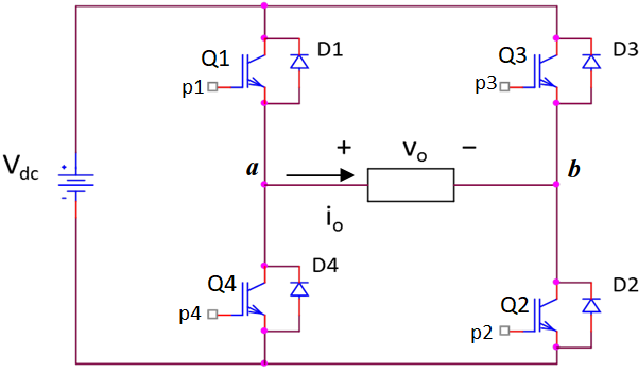
\includegraphics[width=0.45\textwidth]{Images/circuit1.png}
	\label{circuit_1}
\end{figure}

\subsubsection{Μονοφασικός Αντιστροφέας Γέφυρας Τετραγωνικού Παλμού}
\subsubsection{Μονοφασικός Αντιστροφέας Γέφυρας με μονοπολική PWM}
\noindent
Για την παραγωγή της AC τάσης και AC ρεύματος εξόδου, σε αυτή την περίπτωση, δημιουργούνται τετραγωνικοί παλμοί διαφορετικού εύρους μέσω των οποίων, ανάλογα με το εύρος τους, ελέγχεται το πλάτος της τάσης εξόδου.
\noindent\\\\\\
Στην παραπάνω διάταξη τα transistor ενεργοποιούνται με συγκεκριμένο σειρά ώστε οι παλμοί ελέγχου να κατασκευάζουν την επιθυμητή τάση εξόδου εξόδου, ενώ οι δίοδοι χρησιμοποιούνται  για την ροή ρεύματος προς αντίθετη φορά από αυτή των ενεργοποιημένων transistor, λόγω της εναλλασσόμενης μορφής του ρεύματος.

\noindent\\
Για την παραγωγή των παλμών ελέγχου, κατασκευάζεται το επιθυμητό ημιτονοειδές σήμα εξόδου καθώς και ένας τριγωνικός παλμός (Φέρον) πλάτους $V_{dc}$, συχνότητας ίση με την διακοπτική $(m_f \cdot f)$. Συγκρίνοντας το φέρον με το θετικό ημίτονο εξόδου προκύπτουν οι παλμοί ελέγχου των transistor $Q_1$, $Q_4$ ενώ συγκρίνοντάς το με το αρνητικό προκύπτουν οι παλμοί ελέγχου των transistor $Q_2$, $Q_3$, όπως αυτοί φαίνονται στον πίνακα που ακολουθεί:
\begin{table}[h]
	\centering
	\begin{tabular}{ccccc}
		Condition                                     & $Q_1$ & $Q_2$ & $Q_3$ & $Q_4$ \\ \hline
		\multicolumn{1}{c|}{$V_{ref} > V_{carrier}$}  & ON    & -     & -     & OFF   \\
		\multicolumn{1}{c|}{$V_{ref} < V_{carrier}$}  & OFF   & -     & -     & ON    \\
		\multicolumn{1}{c|}{$-V_{ref} > V_{carrier}$} & -     & OFF   & ON    & -     \\
		\multicolumn{1}{c|}{$-V_{ref} < V_{carrier}$} & -     & ON    & OFF   & -    
	\end{tabular}
\end{table}
\noindent\\
Σύμφωνα με τα παραπάνω δεδομένα προκύπτει η τιμή της τάσης στο κόμβο a και στον κόμβο b, εφόσον τα ενεργά transistor δρουν ως βραχυκύκλωμα. Μέσω των τάσεων $V_a$ και $V_b$ η τάση εξόδου στο φορτίο:
\begin{equation}
	V_{out} = V_a - V_b
\end{equation}
\noindent
Τέλος, για την καλύτερη ανάλυση του συστήματος ορίζεται ο δείκτης διαμόρφωσης πλάτους ($m_a$) και ο δείκτης διαμόρφωσης συχνότητας ($m_f$). Ο  $m_a$ ορίζεται ως το πηλίκο μεταξύ του πλάτους του σήματος αναφοράς και του πλάτους του φέροντος και σύμφωνα με την θεωρία, για τιμές μικρότερες της μονάδας επηρεάζει το πλάτης της βασικής αρμονικής ως εξής:
\begin{equation}
	V_1 = m_a \cdot V_{dc}
\end{equation}
Αντίστοιχα, ο $m_f$ ορίζεται ως το πηλίκο μεταξύ της συχνότητας του σήματος αναφοράς και της συχνότητας του φέροντος και σύμφωνα με την θεωρία, αυξάνοντας τον οι αρμονικές του σήματος μετατοπίζονται σε μεγαλύτερες συχνότητες.